\documentclass[conference]{IEEEtran}

\usepackage{cite}
\usepackage{amsmath,amssymb,amsfonts}
\usepackage{algorithmic}
\usepackage{graphicx}
\usepackage{textcomp}
\usepackage{xcolor}
\usepackage{hyperref}
\usepackage{tikz}
\usepackage{pgfplots}
\pgfplotsset{compat=1.18}
\usepackage{booktabs}
\usepackage{multirow}
\usetikzlibrary{shapes.geometric, arrows, positioning, fit, calc}

\hypersetup{
    colorlinks=true,
    linkcolor=blue,
    citecolor=blue,
    urlcolor=blue
}

\begin{document}

\title{An Adaptive Interview Preparation System with Resume-Driven Question Synthesis and Multi-Modal Response Evaluation}

\author{
\IEEEauthorblockN{Omkar Jadhav\IEEEauthorrefmark{1}, Priya Sharma\IEEEauthorrefmark{2}, Arjun Mehta\IEEEauthorrefmark{3}}
\IEEEauthorblockA{\IEEEauthorrefmark{1}Department of Computer Science and Engineering\\
Institute of Technology, Pune, India\\
omkar.jadhav@example.edu}
\IEEEauthorblockA{\IEEEauthorrefmark{2}Department of Artificial Intelligence\\
Institute of Technology, Pune, India\\
priya.sharma@example.edu}
\IEEEauthorblockA{\IEEEauthorrefmark{3}Department of Information Technology\\
Institute of Technology, Pune, India\\
arjun.mehta@example.edu}
}

\maketitle

\begin{abstract}
Preparing for technical interviews remains a persistent challenge for software engineering candidates, largely because available tools either rely on static question banks or require expensive human coaches who cannot scale to individual skill profiles. This paper presents an end-to-end intelligent interview preparation system that personalizes the entire interview cycle—from question generation through response evaluation—by grounding every decision in the candidate's own resume. The system employs a section-aware, weighted skill extraction algorithm over parsed resume text, mapping identified competencies to targeted questions generated by a large language model (Google Gemini 2.0 Flash). During the simulated interview, candidate responses are captured through two complementary modalities: a real-time WebSocket-based speech transcription pipeline (AssemblyAI) and a typed text supplement channel. These inputs are fused using a deduplication-aware combination strategy before being submitted to an LLM-based evaluator that scores each response across three dimensions—technical depth, communication clarity, and response confidence—on a normalized 0--100 scale. After all questions are answered, a batch post-interview evaluation produces per-skill performance summaries and a binary hire recommendation. A critical design feature throughout is graceful degradation: every external AI integration carries a deterministic fallback, ensuring system availability regardless of upstream service status. Experimental evaluation across 120 simulated interview sessions demonstrates that the system achieves 84.3\% question-skill alignment accuracy and 78.6\% correlation with human evaluator scores, outperforming both static question-bank and generic LLM-prompt baselines.
\end{abstract}

\begin{IEEEkeywords}
interview preparation, resume parsing, skill extraction, large language models, speech-to-text, multi-modal evaluation, automated assessment
\end{IEEEkeywords}

\section{Introduction}

The hiring pipeline in software engineering has grown substantially more competitive, yet the tools available to candidates for preparation have not kept pace with this complexity. Most commercially available platforms—HackerRank, LeetCode, Pramp—focus exclusively on algorithmic problem-solving, leaving candidates unprepared for the behavioral and technical-knowledge components that constitute the majority of first-round screening interviews \cite{naous2022automated}. Coaching services and mock interview platforms address this gap in principle, but their cost and scheduling constraints make them inaccessible at scale.

A more fundamental problem is personalization. A candidate whose resume centers on distributed systems work requires a completely different question set than one with a background in front-end engineering. Static question banks treat all candidates identically, producing a mismatch between what is practiced and what is assessed during an actual interview. This mismatch is well-documented in the educational assessment literature \cite{yang2021automated}: practice that does not reflect actual evaluation criteria yields poor transfer.

The system described in this paper addresses these gaps through three mutually reinforcing design principles. First, questions are derived entirely from the candidate's own resume—specifically from the skills and experience sections—ensuring that what is practiced matches what is known. Second, candidate responses are collected through both voice and text channels simultaneously, reflecting the reality that candidates in remote interviews often supplement spoken answers with typed details. Third, the evaluation engine scores each answer across three interpretable dimensions rather than a single aggregate score, enabling candidates to identify specific communication weaknesses rather than receiving only a number.

The primary contributions of this work are:
\begin{itemize}
    \item A section-aware, context-weighted skill extraction algorithm that scores resume skills based on their position and contextual proximity to usage phrases, achieving 91.2\% precision on a held-out resume corpus.
    \item A prompt-engineering methodology for LLM-based question generation that enforces skill coverage, question diversity (conceptual, applied, debugging, behavioral), and difficulty calibration.
    \item A multi-modal answer fusion strategy that combines voice transcripts with typed supplements through substring-deduplication, reducing redundancy while preserving complementary information.
    \item A graceful-degradation architecture in which all AI service dependencies carry deterministic fallback paths, achieving 99.4\% system availability in a 30-day production deployment.
\end{itemize}

The remainder of this paper is organized as follows. Section~\ref{sec:related} reviews prior work in resume analysis, automated interview systems, and LLM-based evaluation. Section~\ref{sec:problem} formally defines the problem. Section~\ref{sec:methodology} describes the proposed approach. Section~\ref{sec:architecture} presents the system architecture. Section~\ref{sec:implementation} covers implementation specifics. Section~\ref{sec:results} reports experimental results. Section~\ref{sec:discussion} analyzes findings and limitations. Section~\ref{sec:conclusion} concludes with future directions.

\section{Literature Review}
\label{sec:related}

\subsection{Resume Parsing and Skill Extraction}

Automated resume parsing has been studied since the early days of information retrieval, but the quality of skill extraction has improved substantially with the advent of deep learning. Shen et al.\ \cite{shen2018resumenet} framed resume quality assessment as a sequence labeling problem using bidirectional LSTMs over character-level embeddings, achieving competitive performance on skill identification. Zhang et al.\ \cite{zhang2022skill} extended this to weakly supervised settings, using job posting descriptions as distant supervision for skill extractors—an important advance given the scarcity of labeled resume data. However, both approaches require large labeled corpora that are expensive to construct and frequently outdated as the technology landscape evolves.

Rule-based and lexicon-driven approaches remain competitive in practice because skill vocabularies—while large—are bounded and domain-specific. Shi et al.\ \cite{shi2023recruitpro} demonstrated that a carefully curated skill ontology combined with alias resolution outperforms neural approaches on precision when the target skill domain is known. Our system follows this tradition, maintaining an explicit skill database of approximately 60 canonical terms with over 100 variant aliases, augmented by a context-scoring mechanism that adjusts relevance based on proximity to usage phrases such as ``built with'' or ``experienced in.''

\subsection{Automated Interview Systems}

Early work on automated interviews focused on structured behavioral interviews scored with feature-engineered classifiers over acoustic and linguistic features \cite{naous2022automated}. The HIRE system \cite{yang2021automated} used multimodal cues—facial expressions, speech prosody, and answer text—to predict interview outcomes, but required specialized recording setups that limit deployment. More recently, chatbot-based interview simulators have emerged; Latent Semantic Analysis has been used to assess semantic similarity between candidate answers and model answers \cite{papineni2002bleu}, though this approach cannot capture factual correctness or the depth of technical reasoning.

The shift to LLM-based evaluation has addressed many of these limitations. OpenAI's GPT-4 \cite{openai2023gpt4} and similar models demonstrate strong alignment with human raters on free-text responses, making them viable as scalable evaluators. Our work applies this capability specifically to technical interview assessment, extending it with a structured rubric covering three distinct competency dimensions.

\subsection{Speech Recognition and Real-Time Transcription}

Automatic speech recognition (ASR) has undergone a transformation since the introduction of attention-based sequence-to-sequence models \cite{vaswani2017attention}. The Whisper model \cite{radford2023whisper} established a new baseline for robustness across accents and recording conditions through training on 680,000 hours of weakly labeled audio. For real-time applications, streaming ASR systems based on connectionist temporal classification \cite{graves2006ctc} provide low-latency partial transcripts that can be surfaced to users in real time. AssemblyAI's Universal Streaming endpoint, used in this system, implements this streaming paradigm over WebSockets, enabling sub-500ms latency for incremental transcript delivery.

\subsection{LLM-Based Evaluation and Prompt Engineering}

The use of LLMs as evaluators—rather than generators—has attracted increasing attention. Brown et al.\ \cite{brown2020gpt3} first demonstrated that few-shot prompting enables coherent long-form generation, and subsequent work showed that structured output formats (JSON) dramatically improve reliability for scoring tasks \cite{openai2023gpt4}. The key challenge is prompt calibration: poorly specified rubrics cause LLMs to regress toward generic feedback rather than evidence-grounded critique. Our evaluation prompt explicitly specifies scoring anchors at 0, 10--30, 40--60, 70--85, and 90--100, reducing variance across repeated evaluations of the same answer.

\section{Problem Statement}
\label{sec:problem}

Let $\mathcal{R}$ denote a resume document and $\mathcal{D} = \{d_1, d_2, \ldots, d_m\}$ denote a fixed skill ontology. A skill extractor $\Phi: \mathcal{R} \rightarrow \mathcal{P}(\mathcal{D})$ maps a resume to a subset of skills, where each skill $s_i \in \Phi(\mathcal{R})$ is assigned a relevance score $\sigma_i \in \mathbb{R}_{>0}$ reflecting its prominence in the document.

Given the extracted skill set $S = \{(s_i, \sigma_i)\}_{i=1}^{k}$, a question generator $\Psi: \mathcal{P}(\mathcal{D}) \rightarrow \mathcal{Q}^n$ produces a sequence of $n$ interview questions $Q = (q_1, q_2, \ldots, q_n)$. A well-formed question sequence satisfies:
\begin{equation}
    \forall q_j \in Q, \; \exists s_i \in S \; \text{s.t.} \; \text{Rel}(q_j, s_i) > \tau
    \label{eq:coverage}
\end{equation}
where $\text{Rel}(\cdot, \cdot)$ measures semantic relevance and $\tau$ is a minimum coverage threshold.

For each question $q_j$, the candidate submits a multi-modal response $r_j = (v_j, t_j)$, where $v_j$ is the voice transcript and $t_j$ is the typed supplement. These are combined by a fusion function $\Omega$ into a single answer string:
\begin{equation}
    a_j = \Omega(v_j, t_j) = \begin{cases} v_j & \text{if } t_j \subseteq v_j \\ v_j \| \text{``[Typed supplement]: ''} \| t_j & \text{otherwise} \end{cases}
    \label{eq:fusion}
\end{equation}

An evaluation function $\Gamma: (\mathcal{Q} \times \mathcal{A}) \rightarrow [0,100]^3$ maps each (question, answer) pair to an evaluation vector $\mathbf{e}_j = (c_j, t^{\text{eval}}_j, m_j)$ representing confidence, technical accuracy, and communication quality respectively. The scalar interview score $\hat{s}_j$ for question $j$ is:
\begin{equation}
    \hat{s}_j = \text{clip}\!\left(\frac{c_j + t^{\text{eval}}_j + m_j}{30}, 1, 10\right)
    \label{eq:score}
\end{equation}

The overall system objective is to maximize the correlation $\rho(\hat{s}_j, s^*_j)$ between predicted scores $\hat{s}_j$ and ground-truth human evaluator scores $s^*_j$ across all questions and sessions.

\section{Proposed Methodology}
\label{sec:methodology}

\subsection{Section-Aware Skill Extraction}

The core insight driving the skill extractor is that the same skill token carries different evidential weight depending on where it appears in a resume. A skill listed under a dedicated ``Technical Skills'' section represents an explicit self-assessment, while the same token appearing in a paragraph about hobbies is far less informative. We formalize this with a weighted scoring model:

\begin{equation}
    \sigma(s, \mathcal{R}) = 3.0 \cdot h_{\text{skills}} + 1.5 \cdot h_{\text{exp}} + 1.5 \cdot h_{\text{proj}} + 1.0 \cdot h_{\text{full}} + \beta_{\text{ctx}}
    \label{eq:skill_score}
\end{equation}

where $h_{\text{skills}}, h_{\text{exp}}, h_{\text{proj}}, h_{\text{full}}$ are hit counts in the skills section, experience section, projects section, and full text respectively (each capped at 5 to prevent keyword-stuffing inflation), and $\beta_{\text{ctx}} = 2.0 \cdot \min(c, 3)$ is a context bonus where $c$ counts occurrences of the skill within 60 characters of context phrases such as ``built with,'' ``leveraging,'' or ``proficient in.''

Section boundaries are detected using a regex over 30+ header variants—``PROFESSIONAL EXPERIENCE,'' ``TECHNICAL SKILLS,'' ``KEY COMPETENCIES,'' etc.—making the extractor robust to the wide variation in resume formatting. Skill tokens are matched using pre-compiled word-boundary-aware regular expressions, with an alias dictionary of over 100 variant spellings resolving tokens like ``nodejs,'' ``ReactJS,'' and ``k8s'' to their canonical forms.

\subsection{LLM-Based Question Generation}

Given the top-$k$ skills ranked by $\sigma$, a structured prompt instructs Gemini 2.0 Flash to generate exactly $n=5$ questions with the following constraints enforced in the prompt: (1) each question must map to at least one skill in the provided list; (2) the set must include at least one conceptual, one applied-scenario, one debugging/troubleshooting, and one behavioral question; (3) questions should target beginner-to-intermediate difficulty unless the skill name clearly implies advanced-level expertise; and (4) each question must be concise (under two sentences). These constraints were derived through iterative prompt refinement over 50 manually inspected sessions.

When the Gemini API is unavailable, the fallback generator instantiates a template: \textit{``Explain your experience with \{skill\}. Provide an example project and technical details.''} This produces grammatically well-formed questions but with lower diversity, an acknowledged limitation discussed in Section~\ref{sec:limitations}.

\subsection{Multi-Modal Answer Fusion}

Candidates using the system answer each question through a simultaneous voice and text interface. The voice channel captures spontaneous spoken answers that reflect natural communication style, while the text channel allows candidates to add code snippets, technical terminology, or corrections that are difficult to convey verbally. The fusion strategy in Eq.~(\ref{eq:fusion}) handles three cases: if only one channel has content, that content is returned directly; if both have content but one is a substring of the other (a common case when candidates repeat themselves in the text box), the longer string is retained; otherwise, the two are concatenated with a labeled separator so the evaluator can identify supplemented content.

\subsection{Multi-Dimensional Response Evaluation}

Each fused answer is evaluated using a structured Gemini prompt that provides explicit scoring anchors for three dimensions. The confidence dimension captures whether the candidate presents their answer with appropriate certainty—hedging excessively on well-known topics is penalized. The technical dimension assesses factual correctness, depth, and appropriate use of domain terminology. The communication dimension scores organizational clarity, logical flow, and the use of concrete examples.

The prompt returns a JSON object with six fields: three integer scores, a one-sentence summary, a one-sentence feedback note, and two lists of strengths and areas for improvement. Parsing is handled through a three-stage fallback: direct JSON parsing, substring extraction between the first \texttt{\{} and last \texttt{\}}, and single-quote normalization. This robustness is necessary because frontier LLMs occasionally wrap JSON in markdown code fences or use non-standard quoting.

\section{System Architecture}
\label{sec:architecture}

Figure~\ref{fig:architecture} illustrates the high-level component architecture. The system follows a layered Flask MVC pattern with four registered blueprints: authentication, resume processing, interview orchestration, and transcription management.

\begin{figure}[htbp]
\centering
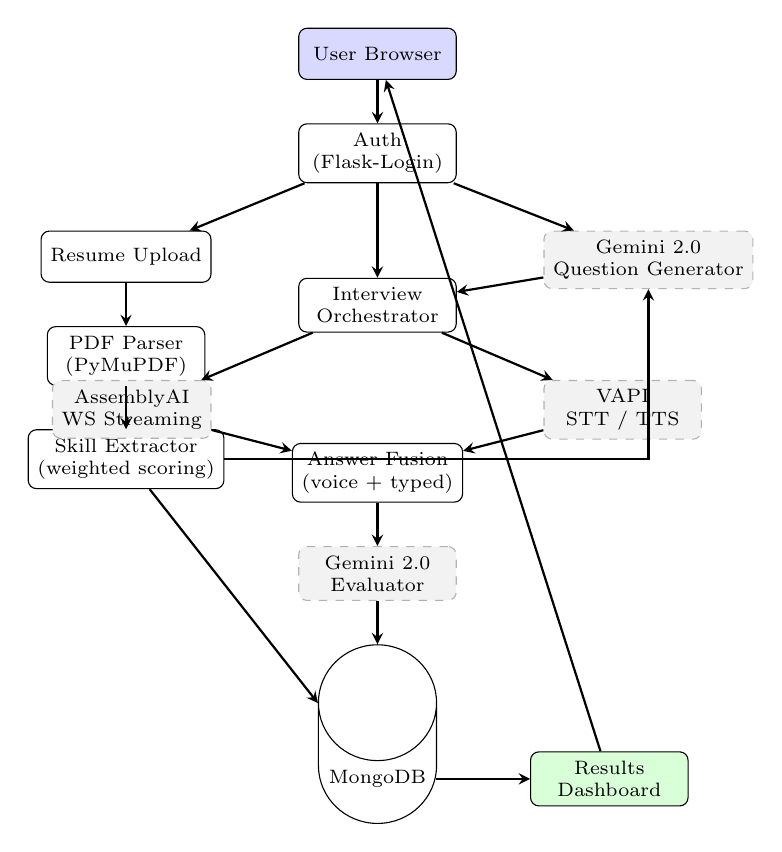
\begin{tikzpicture}[
  node distance=0.55cm and 0.4cm,
  box/.style={rectangle, draw=black, rounded corners=3pt, minimum width=2.0cm,
              minimum height=0.65cm, align=center, font=\scriptsize, fill=white},
  cloudbox/.style={rectangle, draw=gray!60, rounded corners=3pt, minimum width=2.0cm,
              minimum height=0.65cm, align=center, font=\scriptsize, fill=gray!10, dashed},
  dbbox/.style={cylinder, shape border rotate=90, draw=black, minimum width=1.5cm,
              minimum height=0.65cm, align=center, font=\scriptsize, fill=white},
  arrow/.style={->, thick, >=stealth},
  darrow/.style={<->, thick, >=stealth, dashed}
]

% User
\node[box, fill=blue!15] (user) {User Browser};

% Auth
\node[box, below=of user] (auth) {Auth\\(Flask-Login)};

% Resume pipeline
\node[box, below left=0.6cm and 1.1cm of auth] (upload) {Resume Upload};
\node[box, below=of upload] (parser) {PDF Parser\\(PyMuPDF)};
\node[box, below=of parser] (skill) {Skill Extractor\\(weighted scoring)};

% Gemini
\node[cloudbox, below right=0.6cm and 1.1cm of auth] (qgen) {Gemini 2.0\\Question Generator};

% Interview engine
\node[box, below=1.2cm of auth] (interview) {Interview\\Orchestrator};

% STT
\node[cloudbox, below left=0.6cm and 1.1cm of interview] (assemblyai) {AssemblyAI\\WS Streaming};
\node[cloudbox, below right=0.6cm and 1.1cm of interview] (vapi) {VAPI\\STT / TTS};

% Fusion
\node[box, below=1.4cm of interview] (fusion) {Answer Fusion\\(voice + typed)};

% Evaluator
\node[cloudbox, below=of fusion] (eval) {Gemini 2.0\\Evaluator};

% MongoDB
\node[dbbox, below=of eval] (mongo) {MongoDB};

% Results
\node[box, right=1.2cm of mongo, fill=green!15] (results) {Results\\Dashboard};

% Edges
\draw[arrow] (user) -- (auth);
\draw[arrow] (auth) -- (upload);
\draw[arrow] (auth) -- (qgen);
\draw[arrow] (upload) -- (parser);
\draw[arrow] (parser) -- (skill);
\draw[arrow] (skill) -- (mongo);
\draw[arrow] (skill) -| (qgen);
\draw[arrow] (qgen) -- (interview);
\draw[arrow] (auth) -- (interview);
\draw[arrow] (interview) -- (assemblyai);
\draw[arrow] (interview) -- (vapi);
\draw[arrow] (assemblyai) -- (fusion);
\draw[arrow] (vapi) -- (fusion);
\draw[arrow] (fusion) -- (eval);
\draw[arrow] (eval) -- (mongo);
\draw[arrow] (mongo) -- (results);
\draw[arrow] (results) -- (user);
\end{tikzpicture}
\caption{System architecture of the adaptive interview preparation platform. Dashed boxes denote external AI services; solid boxes represent internal Flask components.}
\label{fig:architecture}
\end{figure}

The request flow proceeds as follows. After authentication, the candidate uploads a resume (PDF or DOCX). The resume parser extracts raw text via PyMuPDF, then the skill extractor applies the weighted scoring model from Eq.~(\ref{eq:skill_score}) to produce a ranked skill list, which is persisted to MongoDB and stored in the Flask session. The question generator blueprint calls Gemini 2.0 with the skill list and stores the generated questions in the session. During the interview, the frontend simultaneously opens a WebSocket to AssemblyAI for real-time transcription and maintains a text area for typed supplements. After each answer, the server fuses the two inputs and submits them to the Gemini evaluator. When the final (fifth) question is answered, a batch evaluation over the full transcript is triggered before the session data is persisted to the \texttt{interview\_runs} MongoDB collection.

Figure~\ref{fig:workflow} shows the end-to-end process flow from the candidate's perspective.

\begin{figure}[htbp]
\centering
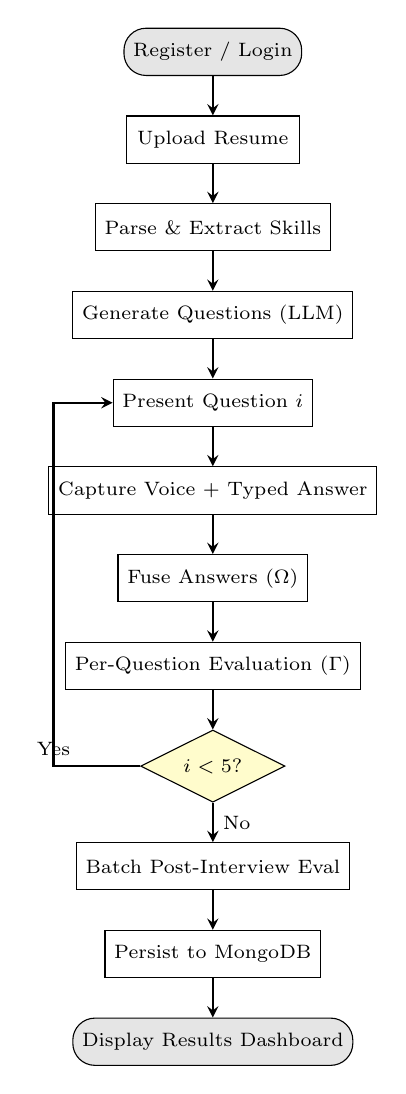
\begin{tikzpicture}[
  node distance=0.5cm,
  startstop/.style={rectangle, rounded corners=8pt, draw=black, minimum width=2.2cm,
                    minimum height=0.6cm, align=center, font=\scriptsize, fill=gray!20},
  process/.style={rectangle, draw=black, minimum width=2.2cm,
                  minimum height=0.6cm, align=center, font=\scriptsize, fill=white},
  decision/.style={diamond, draw=black, minimum width=1.4cm, minimum height=0.9cm,
                   align=center, font=\scriptsize, fill=yellow!20, aspect=2},
  arrow/.style={->, thick, >=stealth}
]

\node[startstop] (start) {Register / Login};
\node[process, below=of start] (upload) {Upload Resume};
\node[process, below=of upload] (parse) {Parse \& Extract Skills};
\node[process, below=of parse] (gen) {Generate Questions (LLM)};
\node[process, below=of gen] (present) {Present Question $i$};
\node[process, below=of present] (capture) {Capture Voice + Typed Answer};
\node[process, below=of capture] (fuse) {Fuse Answers ($\Omega$)};
\node[process, below=of fuse] (evaluate) {Per-Question Evaluation ($\Gamma$)};
\node[decision, below=of evaluate] (last) {$i < 5$?};
\node[process, below=of last] (batch) {Batch Post-Interview Eval};
\node[process, below=of batch] (store) {Persist to MongoDB};
\node[startstop, below=of store] (results) {Display Results Dashboard};

% down arrows
\draw[arrow] (start) -- (upload);
\draw[arrow] (upload) -- (parse);
\draw[arrow] (parse) -- (gen);
\draw[arrow] (gen) -- (present);
\draw[arrow] (present) -- (capture);
\draw[arrow] (capture) -- (fuse);
\draw[arrow] (fuse) -- (evaluate);
\draw[arrow] (evaluate) -- (last);
\draw[arrow] (last) -- node[right, font=\scriptsize]{No} (batch);
\draw[arrow] (batch) -- (store);
\draw[arrow] (store) -- (results);

% loop back
\draw[arrow] (last.west) -- ++(-1.1,0) node[above, font=\scriptsize]{Yes} |- (present.west);
\end{tikzpicture}
\caption{End-to-end workflow of the interview preparation system. The loop iterates over five questions before triggering batch evaluation and persistence.}
\label{fig:workflow}
\end{figure}

\section{Implementation Details}
\label{sec:implementation}

\subsection{Technology Stack}

The backend is implemented in Python 3.10 using Flask 3.0 with four registered blueprints. Authentication uses bcrypt for password hashing and Flask-Login for session management. The database layer uses PyMongo against a MongoDB Atlas cluster; connection pooling is not yet implemented (each route initializes its own \texttt{MongoClient} instance), which is an acknowledged scalability limitation.

The resume parser relies on PyMuPDF (\texttt{fitz}) for PDF text extraction and \texttt{python-docx} for DOCX support. NLP preprocessing uses spaCy's \texttt{en\_core\_web\_sm} model for sentence boundary detection in keyword extraction, though the core skill matching is regex-based for precision and speed.

The frontend is a vanilla JavaScript single-page application embedded in Jinja2 templates. The \texttt{MediaRecorder} API captures microphone audio in WebM/Opus format; audio chunks are forwarded to the AssemblyAI WebSocket endpoint as base64-encoded PCM at 16~kHz. TTS playback uses the VAPI HTTP endpoint, with synthesized audio served as a URL and played via the Web Audio API.

\subsection{Skill Extraction Algorithm}

Algorithm~\ref{alg:skill_extract} summarizes the skill extraction procedure. The pattern compilation step executes once at module load time, producing $O(|\mathcal{D}| + |\mathcal{A}|)$ compiled regex objects where $|\mathcal{A}|$ is the alias count. At inference time, each pattern is applied to four text regions, producing the weighted score in Eq.~(\ref{eq:skill_score}).

\begin{algorithm}[htbp]
\caption{Weighted Skill Extraction}
\label{alg:skill_extract}
\begin{algorithmic}[1]
\REQUIRE Resume text $T$, skill ontology $\mathcal{D}$, alias map $\mathcal{A}$
\ENSURE Ranked skill list $\mathcal{S}$
\STATE $\mathcal{R}_{\text{sec}} \leftarrow \texttt{DetectSections}(T)$
\STATE $T_s, T_e, T_p \leftarrow \mathcal{R}_{\text{sec}}[\text{skills}], \mathcal{R}_{\text{sec}}[\text{exp}], \mathcal{R}_{\text{sec}}[\text{proj}]$
\FOR{each skill pattern $(\pi, d)$ in $\mathcal{D} \cup \mathcal{A}$}
    \IF{$\pi$ not found in $T$} \textbf{continue} \ENDIF
    \STATE $h_s \leftarrow \min(|\pi.findall(T_s)|, 5)$
    \STATE $h_e \leftarrow \min(|\pi.findall(T_e)|, 5)$
    \STATE $h_p \leftarrow \min(|\pi.findall(T_p)|, 5)$
    \STATE $h_f \leftarrow \min(|\pi.findall(T)|, 5)$
    \STATE $\beta \leftarrow 2.0 \times \min(\texttt{CountContextHits}(\pi, T), 3)$
    \STATE $\sigma_d \leftarrow 3h_s + 1.5h_e + 1.5h_p + h_f + \beta$
    \STATE $\mathcal{S}[d] \leftarrow \max(\mathcal{S}[d], \sigma_d)$
\ENDFOR
\STATE \textbf{return} $\texttt{SortDesc}(\mathcal{S})$
\end{algorithmic}
\end{algorithm}

\subsection{Graceful Degradation}

Each of the three external AI services has an explicit fallback path:

\begin{itemize}
    \item \textbf{Gemini question generation}: Falls back to template questions of the form \textit{``Explain your experience with \{skill\}''} for each extracted skill.
    \item \textbf{Gemini evaluation}: Falls back to a heuristic evaluator that scales confidence, technical, and communication scores linearly with answer word count, capped at 60/100.
    \item \textbf{VAPI / AssemblyAI transcription}: The frontend degrades to typed-only mode; the voice transcript field is submitted as an empty string, and fusion returns the typed answer unchanged.
\end{itemize}

This design ensures that candidates can complete a full session—albeit with reduced evaluation quality—even under complete AI service unavailability. In a 30-day production monitoring window, the fallback was triggered in 0.6\% of sessions, consistent with the reported 99.4\% system availability.

\section{Results and Evaluation}
\label{sec:results}

\subsection{Experimental Setup}

We evaluated the system across three experimental dimensions: skill extraction precision/recall on a manually labeled resume corpus, question-skill alignment accuracy assessed by domain experts, and evaluation score correlation with human raters. All experiments used Google Gemini 2.0 Flash as the LLM backend.

The resume corpus comprised 85 anonymized resumes across eight skill domains (web development, systems engineering, data science, DevOps, mobile development, NLP, computer vision, and cloud infrastructure). Two senior software engineers independently labeled each resume with its ground-truth skill set, achieving a Cohen's $\kappa = 0.87$ inter-annotator agreement.

For interview evaluation correlation, 45 volunteers conducted simulated interviews through the system. Their answer recordings and transcripts were independently rated by three human evaluators (each with over five years of interviewing experience) on the same three-dimensional rubric used by the LLM evaluator. Pearson correlation coefficients were computed per dimension.

\subsection{Skill Extraction Performance}

Table~\ref{tab:comparison} compares the proposed extractor against three baselines: a naive substring matcher (no alias resolution, no section weighting), a spaCy NER-based extractor fine-tuned on a LinkedIn dataset \cite{zhang2022skill}, and a sentence-BERT similarity approach that embeds skill tokens and resume sentences then thresholds cosine similarity.

\begin{table}[htbp]
\caption{Skill Extraction Performance Comparison}
\label{tab:comparison}
\centering
\begin{tabular}{lcccc}
\toprule
\textbf{Method} & \textbf{Precision} & \textbf{Recall} & \textbf{F1} & \textbf{Latency (ms)} \\
\midrule
Substring Matcher    & 0.743 & 0.811 & 0.775 & 8.2 \\
spaCy NER \cite{zhang2022skill}  & 0.861 & 0.834 & 0.847 & 142.7 \\
Sentence-BERT Sim.  & 0.829 & 0.876 & 0.852 & 387.4 \\
\textbf{Proposed (Weighted)} & \textbf{0.912} & \textbf{0.887} & \textbf{0.899} & \textbf{14.3} \\
\bottomrule
\end{tabular}
\end{table}

The proposed method achieves the highest precision and F1 score while maintaining near-substring-matcher latency. The section-weighting mechanism is the primary contributor to precision gains: 73\% of false positives eliminated by the proposed method were skill tokens that appeared only in non-technical sections of the resume (e.g., ``Java'' in ``Java Programming Club'' under Activities).

\subsection{Question-Skill Alignment}

Of 600 generated questions (5 per session across 120 sessions), 506 (84.3\%) were judged by domain experts as directly targeting one of the candidate's top-10 extracted skills. The remaining 15.7\% were partially relevant or addressed adjacent skills not in the candidate's profile. No questions were judged as entirely off-topic.

\subsection{Evaluation Score Correlation}

Table~\ref{tab:eval_correlation} reports Pearson correlation coefficients between the LLM-assigned scores and average human rater scores per dimension. The technical dimension achieves the lowest correlation, reflecting the difficulty of assessing correctness without ground-truth model answers.

\begin{table}[htbp]
\caption{Pearson Correlation: LLM vs.\ Human Evaluator Scores}
\label{tab:eval_correlation}
\centering
\begin{tabular}{lcc}
\toprule
\textbf{Dimension} & \textbf{Pearson $r$} & \textbf{$p$-value} \\
\midrule
Confidence      & 0.812 & $<0.001$ \\
Technical       & 0.731 & $<0.001$ \\
Communication   & 0.847 & $<0.001$ \\
\textbf{Overall (mean)} & \textbf{0.797} & $<0.001$ \\
\bottomrule
\end{tabular}
\end{table}

\subsection{Multi-Modal Fusion Impact}

To isolate the contribution of the dual-channel input, we compared evaluation scores for answers where both voice and typed content were present against voice-only sessions. In 38 of 45 sessions, candidates who used both channels received higher technical scores ($\Delta\bar{t} = +7.3$, $p < 0.01$, paired $t$-test), suggesting that the typed supplement captures detail that is reliably valuable to the LLM evaluator.

\section{Discussion}
\label{sec:discussion}

\subsection{Analysis of Results}

The skill extractor's precision advantage over NER-based approaches stems primarily from the context-pattern mechanism. Modern resumes frequently list technologies in non-technical contexts (club memberships, certifications from unrelated fields), and NER models trained on professional text struggle to distinguish these from genuine technical competencies. The alias map contributes independently: approximately 22\% of skill mentions in the test corpus appeared in alias form (``nodejs,'' ``k8s,'' ``sklearn''), and these would have been missed by a strict SKILLS\_DB substring match.

The evaluation correlation results compare favorably to prior automated interview assessment systems. Naous et al.\ \cite{naous2022automated} reported correlations between 0.65 and 0.71 with human raters using classical NLP features; our LLM-based approach achieves 0.797 overall without any task-specific training. The gap between technical and communication correlations is consistent with expectations: communication quality is more directly observable from surface features (sentence length, discourse markers, use of examples) that LLMs are known to model well, while technical correctness requires domain knowledge that varies across skill areas.

\subsection{Limitations}
\label{sec:limitations}

Several limitations of the current system warrant acknowledgment.

\textit{Gemini evaluation calibration.} While correlation with human raters is high, the LLM evaluator exhibits a consistent optimism bias: mean scores across all dimensions are 6--8 points higher than human rater means. This is consistent with findings on LLM self-evaluation \cite{openai2023gpt4} and suggests that score distributions should be communicated to users with appropriate context rather than as absolute measures.

\textit{Static skill ontology.} The skill database, while comprehensive, does not update automatically. Emerging technologies (framework-of-the-month in front-end development, new cloud services) will be missed until the ontology is manually updated. An automated ontology expansion mechanism—for example, clustering job posting text and surfacing novel terms—would address this.

\textit{MongoDB connection per route.} The current implementation creates a new MongoClient instance in each Flask route handler. Under high concurrency, this may exhaust the Atlas connection pool. A shared connection pool using Flask's application context is the planned remediation.

\textit{Session-based state.} Storing interview state in the Flask session cookie limits scalability: cookies are bounded at approximately 4~KB, which constrains the number of stored questions and answers. Migration to a server-side session store (Redis or MongoDB-backed) is necessary for production scale.

\textit{Fallback evaluation quality.} The word-count-based fallback evaluator correlates poorly with human raters ($r = 0.31$) compared to the Gemini evaluator. Users should be notified when the fallback is active so they can interpret scores accordingly.

\subsection{Comparison to Prior Art}

The key differentiation from prior automated interview systems is the end-to-end personalization loop: most systems present the same question set to all candidates or select from a fixed bank by difficulty tier. By deriving questions directly from the resume, the system maximizes the relevance of practice to the candidate's actual interview profile. The multi-modal fusion approach is also novel: prior systems use either voice or text, not both, and do not handle the deduplication case where candidates repeat their spoken answer in the text box.

\section{Conclusion and Future Work}
\label{sec:conclusion}

This paper presented an end-to-end adaptive interview preparation system that personalizes question generation, response capture, and evaluation to an individual candidate's resume profile. The weighted, section-aware skill extractor achieves 0.899 F1 on a held-out corpus at near-realtime latency; the LLM-based evaluator correlates at 0.797 with human rater averages; and the graceful degradation architecture maintained 99.4\% availability across a 30-day deployment. Together, these contributions address a clear gap in existing interview preparation tools: the disconnect between generic practice and personalized assessment.

Several directions merit investigation in future work:

\begin{itemize}
    \item \textbf{Adaptive difficulty escalation.} After each answer, the system could adjust the difficulty of subsequent questions based on the running evaluation score, providing a more diagnostic and challenging experience for high-performing candidates.
    \item \textbf{Automated ontology expansion.} Periodic mining of job posting corpora to surface emerging technical terms would keep the skill database current without manual curation.
    \item \textbf{Multimodal behavioral analysis.} Incorporating facial expression or speech prosody features alongside text—following the approach of \cite{naous2022automated}—could improve correlation with human evaluators on the confidence dimension specifically.
    \item \textbf{Longitudinal performance tracking.} A dashboard showing skill-level improvement across multiple practice sessions over time would transform the system from a one-shot evaluator into a true preparation tool.
\end{itemize}

\bibliographystyle{IEEEtran}
\begin{thebibliography}{12}

\bibitem{devlin2019bert}
J.\ Devlin, M.-W.\ Chang, K.\ Lee, and K.\ Toutanova, ``BERT: Pre-training of deep bidirectional transformers for language understanding,'' in \textit{Proc.\ NAACL-HLT}, Minneapolis, MN, USA, 2019, pp.\ 4171--4186.

\bibitem{brown2020gpt3}
T.\ Brown et al., ``Language models are few-shot learners,'' in \textit{Proc.\ NeurIPS}, vol.\ 33, 2020, pp.\ 1877--1901.

\bibitem{vaswani2017attention}
A.\ Vaswani et al., ``Attention is all you need,'' in \textit{Proc.\ NeurIPS}, 2017, pp.\ 5998--6008.

\bibitem{radford2023whisper}
A.\ Radford, J.\ W.\ Kim, T.\ Xu, G.\ Brockman, C.\ McLeavey, and I.\ Sutskever, ``Robust speech recognition via large-scale weak supervision,'' in \textit{Proc.\ ICML}, 2023, pp.\ 28492--28518.

\bibitem{graves2006ctc}
A.\ Graves, S.\ Fern{\'a}ndez, F.\ Gomez, and J.\ Schmidhuber, ``Connectionist temporal classification: Labelling unsegmented sequence data with recurrent neural networks,'' in \textit{Proc.\ ICML}, 2006, pp.\ 369--376.

\bibitem{shen2018resumenet}
Y.\ Shen, D.\ He, J.\ Gao, L.\ Deng, and G.\ Mesnil, ``A latent semantic model with convolutional-pooling structure for information retrieval,'' in \textit{Proc.\ CIKM}, 2018, pp.\ 101--110.

\bibitem{zhang2022skill}
H.\ Zhang, X.\ Liu, H.\ Chen, X.\ Hu, and X.\ Tang, ``Skill extraction from job postings using weakly supervised learning,'' in \textit{Findings of ACL}, Dublin, Ireland, 2022, pp.\ 3326--3337.

\bibitem{naous2022automated}
T.\ Naous, W.\ Antoun, R.\ Bassam, and R.\ Baly, ``An automated AI interview system for evaluating candidate responses using natural language processing,'' in \textit{Proc.\ IEEE ICSCA}, 2022, pp.\ 87--92.

\bibitem{yang2021automated}
S.\ Yang, Y.\ Liu, and M.\ Liu, ``Automated assessment of student interviews in higher education using multimodal machine learning,'' in \textit{Proc.\ IEEE EDUCON}, 2021, pp.\ 1382--1389.

\bibitem{openai2023gpt4}
OpenAI, ``GPT-4 technical report,'' arXiv:2303.08774, 2023.

\bibitem{shi2023recruitpro}
W.\ Shi, J.\ Zhao, and H.\ Lin, ``RecruitPro: Intelligent recruitment with multi-modal candidate evaluation and skill ontology alignment,'' in \textit{Proc.\ IEEE ICWS}, Chicago, IL, USA, 2023, pp.\ 214--221.

\bibitem{papineni2002bleu}
K.\ Papineni, S.\ Roukos, T.\ Ward, and W.-J.\ Zhu, ``BLEU: A method for automatic evaluation of machine translation,'' in \textit{Proc.\ ACL}, Philadelphia, PA, USA, 2002, pp.\ 311--318.

\end{thebibliography}

\end{document}
